
% Segundo capítulo deste trabalho.
%--------------------------------------
\chapter{Exemplos de escrita em \LaTeX}
\label{cap2}

Neste capítulo são apresentados alguns exemplos que ajudam na elaboração e na organização de um documento escrito em \LaTeX. 

Na Secção \ref{cap2:sec_listas} são apresentados exemplos de listas com recurso aos comandos \textit{enumerate} e \textit{itemize}.  A utilização de símbolos em \LaTeX \ é exemplificada na Secção \ref{cap2:sec_simbolos}, onde está incluída uma nota de rodapé. Na Secção \ref{cap2:sec_def} são apresentadas definições, exemplos e proposições com o devido destaque. Equações e matrizes são descritas na Secção \ref{cap2:sec_equa}. Nas secções \ref{cap2:sec_tabelas} e \ref{cap2:sec_figuras} são apresentados exemplos de como definir uma tabela e de como incluir uma figura no documento, com a sua referência ao longo do texto. 

Fica a sugestão de apresentar uma pequena descrição do conteúdo de cada capítulo após a escrita do título do capítulo - como foi aqui ilustrado.

\section{Listas}\label{cap2:sec_listas}

    Segue um exemplo de um \textit{enumerate}:
    \begin{enumerate}
    	\item Primeiro item;
    	\item Segundo item;
    	\item Terceiro item.	
    \end{enumerate}
    
    Segue um exemplo de um \textit{itemize}:   
    \begin{itemize}
    	\item Primeiro item;
    	\item Segundo item;
    	\item Terceiro item.
    \end{itemize}
    
\section{Símbolos}\label{cap2:sec_simbolos}

    Alguns exemplos de símbolos gregos são $\Psi$, $\phi$, $\Theta$, $\theta$, $\mu$, $\rho$. Alguns símbolos matemáticos muitas vezes utilizados são os seguintes $\pi$, $\Rightarrow$, $\rightarrow$, $\infty$, $\geq$, $\neq$.

\subsection{Notas de rodapé}

    Para colocar uma nota de rodapé no texto basta colocar o respetivo texto dentro do comando \verb|\footnote|. Por exemplo\footnote{Exemplo de uma nota de rodapé.}.

\section{Etiquetas e respetiva referenciação no texto}

    Aquando da escrita de um documento é, por vezes, necessário referenciar um capítulo, uma secção, uma tabela, uma figura ou uma equação. Para o efeito deve-se utilizar o comando \verb|\label| junto ao elemento a referenciar e o comando \verb|\ref| para fazer a sua chamada no texto.

\section{Definições, exemplos e proposições}
    \label{cap2:sec_def}
    
    \begin{definition}
    Uma equação diferencial diz-se {\bf ordinária} se a
    função incógnita depende apenas de uma variável.
    \end{definition}
    
    \bigskip % para fazer um espaço na vertical
    
    \begin{example}
    São exemplos de equações diferenciais ordinárias as seguintes equações:
    \begin{enumerate}
    \item[(1)]
    $L\frac{d^2Q(t)}{dt^2}+R\frac{dQ(t)}{dt}+\frac{1}{C}Q(t)=E(t)$;
    \item[(2)] $L\frac{dI(t)}{dt}+RI(t)=E(t)$.
    \end{enumerate}
    \end{example}
    
   \bigskip
    
    \begin{proposition}
    Em qualquer triângulo retângulo, o quadrado do comprimento da hipotenusa é igual à soma dos quadrados dos comprimentos dos catetos.  
    \end{proposition}
    
\section{Equações e matrizes}
    \label{cap2:sec_equa}
    
    Nesta secção apresenta-se um exemplo de como definir uma equação numerada bem como a sua referenciação no texto.
    
    A velocidade em cada tecido $v_i,\, i=c,r,v$, pode ser definida por
    
    \begin{equation} 
        \label{Darcy_crv}
        \left\{
        \begin{array}{l}
            v_i=-\frac{k_i}{\mu_i}\nabla p_i \mbox{ in } \Omega_i\times (0,T],\\
            \nabla. v_i=0 \mbox{ in } \Omega_i\times (0,T], \quad i=c,r,v.
        \end{array}
        \right.
    \end{equation}
    
    Na Equação (\ref{Darcy_crv}), $k_i$ representa a permeabilidade do tecido e $\mu_i$ representa a viscosidade do fluido. 
    
    Um exemplo de uma equação centrada no texto sem numeração apresenta-se de seguida.
    
    $$ \gamma_r=\left\{
        \begin{array}{l}
            \gamma_{r,1}  \mbox{ in } \Omega_{r,1},\\
            \gamma_{r,2}  \mbox{ in } \Omega_{r,2}.
        \end{array}
        \right. $$
    
    Um exemplo de uma matriz quadrada é
        \begin{equation}
        M_{3,3}=\left[ \begin{array}{ccc}
                  1&2&3\\
                  4&5&6\\
                  7&8&9
                \end{array}
            \right].\label{matriz}
        \end{equation}     
    A Matriz (\ref{matriz}) tem ordem três. Pode-se  definir uma matriz arbitrariamente grande como, por exemplo, a matriz tridiagonal que se segue:
    
    $$A=\frac{1}{\Delta x^2}\left[ 
        \begin{array}{ccccccc}
               -2\alpha & \alpha-\frac{\beta\Delta x}{2} & 0 & 0 & \cdots & 0 & 0 \\
               \alpha-\frac{\beta\Delta x}{2} & -2\alpha & \alpha+\frac{\beta\Delta x}{2} & 0 & \cdots & 0 & 0 \\
               0 & \alpha-\frac{\beta\Delta x}{2} & -2\alpha & \alpha+\frac{\beta\Delta x}{2} & \cdots & 0 & 0 \\
               \vdots & \vdots & \vdots  & \vdots & \ddots & \ddots & \vdots \\
               0 & 0 & 0 & 0& \cdots& -2\alpha & \alpha+\frac{\beta\Delta x}{2} \\
               0 & 0 & 0 & 0& \cdots& 0 & -2\alpha 
        \end{array}
    \right].$$
    
\section{Tabelas}
    \label{cap2:sec_tabelas}
    
    Segue-se um exemplo de uma tabela em que o conteúdo da primeira coluna está alinhado à esquerda e em que o conteúdo das restantes colunas está centrado, Tabela~\ref{tab_sem_separadores}.  Cada tabela deve ter um título/legenda,  sendo possível associar-lhe uma referência para ser identificada ao longo do texto.
    
    \begin{table}[htp]
    \caption{\small Um exemplo de uma tabela.}
    \label{tab_sem_separadores}
    \centering
    	\begin{tabular}{l|ccc} \hlinewd{2pt}
    		Comparação   & Vítreo & Retina & Coróide \\ 
                \hline
    		SCS com Iont. \textit{vs} No Iont. &  20\% & 7\%&1\% \\
    		SRS com Iont. \textit{vs} No Iont. & 45\% & 14\%&8\% \\
    		SCS com Iont. \textit{vs} Intravitreal &-80\% & 150\% & 2000\% \\
    		SRS com Iont. \textit{vs} Intravitreal & -90\% & 1002\% & 2300\% \\  
    		\hlinewd{2pt}
    	\end{tabular}
    \end{table}
    
    Um exemplo de tabela com separadores entre colunas e todas as celulas centradas apresenta-se na Tabela~\ref{tab_com_separadores}.
    
    \begin{table}[htp]
    \caption{\small Outro exemplo de uma tabela.} 
    \label{tab_com_separadores}
    \centering
    		\begin{tabular}{c|c|c} 
                    \hlinewd{2pt}
    			Tipo de administração & Concentração máxima & Instante \\        \hline
    			SCS com Iont & 0.0034 & 19.7  \\
    			SRS com Iont & 0.0034 & 32  \\
    			Injeção IVI  & 0.0055 & 36.7 \\
    			\hlinewd{2pt}
    		\end{tabular}
    \end{table}
    
    No endereço \verb|https://www.tablesgenerator.com/| poderá encontrar uma forma automatizada de gerar tabelas em \LaTeX.
    
\section{Figuras}
\label{cap2:sec_figuras}

    Para inserir uma figura no texto (em formato PNG) pode ser utilizado o comando \verb|\includegraphics|. É também possível definir com este comando uma etiqueta que permite referenciar a figura no texto, assim como fornecer a legenda da figura.

    \begin{figure}[htp]
    	\centering	
            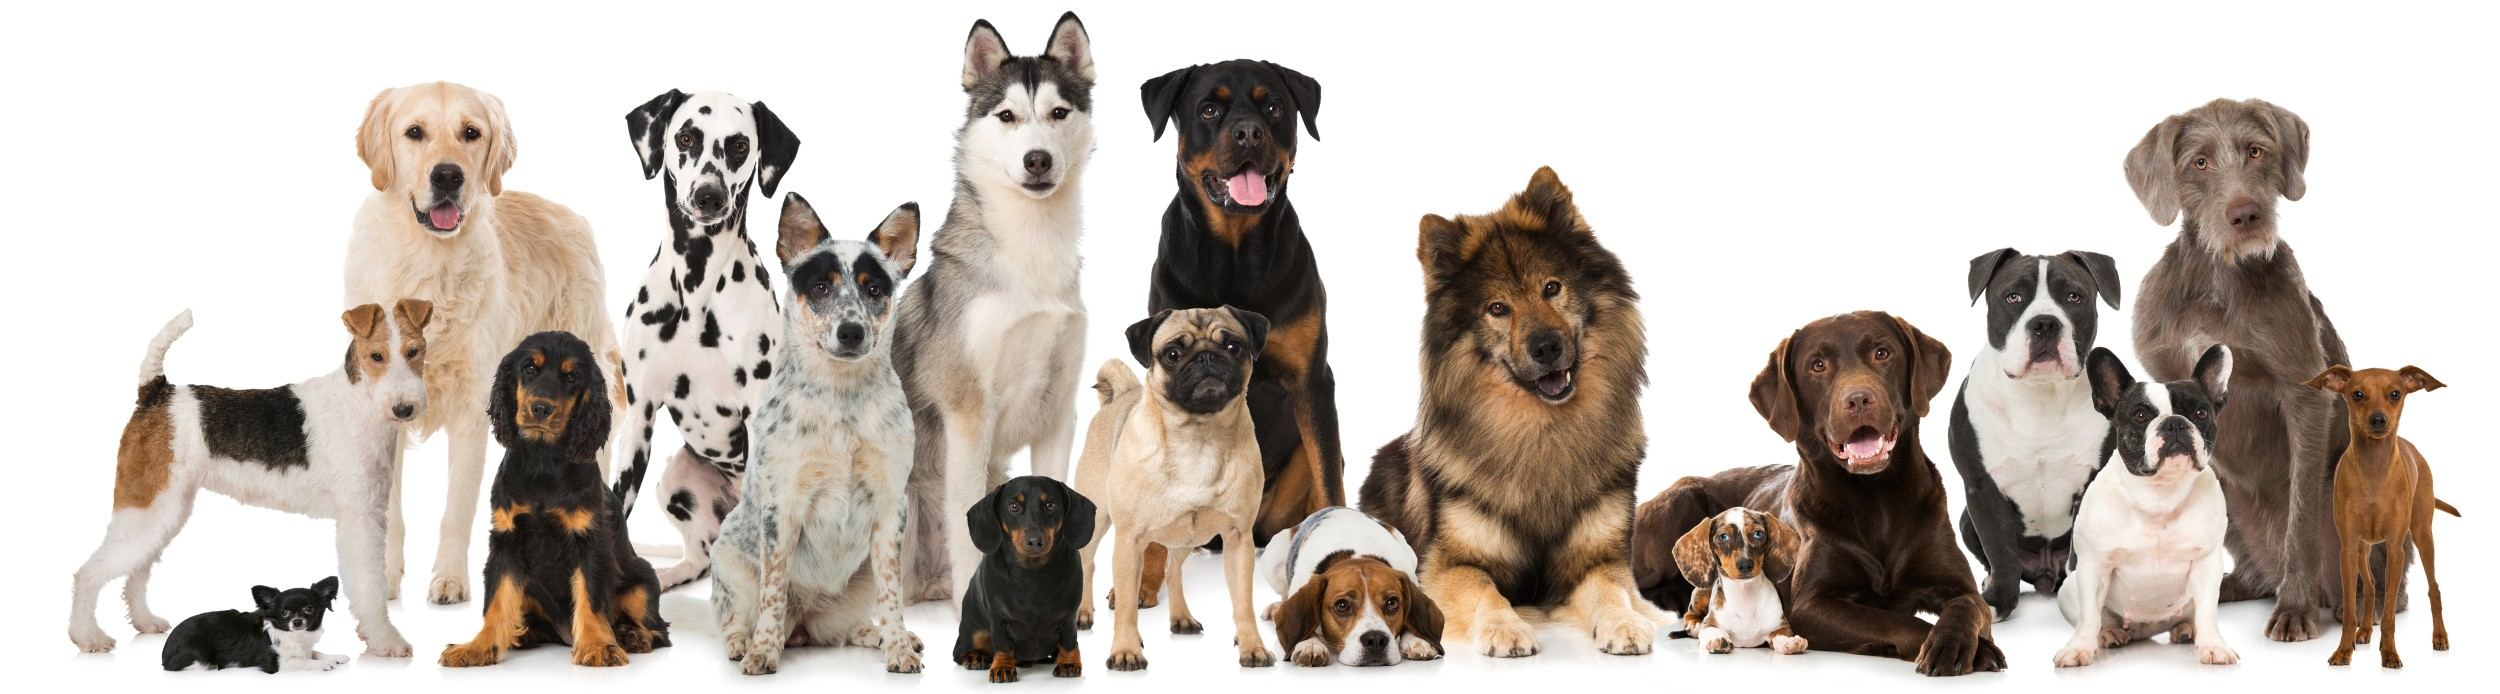
\includegraphics[width=0.8\textwidth]{Figuras/caes}
            \caption{\small Algumas raças caninas.}
    	\label{fig_caes_sem_foot}
    \end{figure}
    
    \begin{figure}[htp]
    	\centering
    	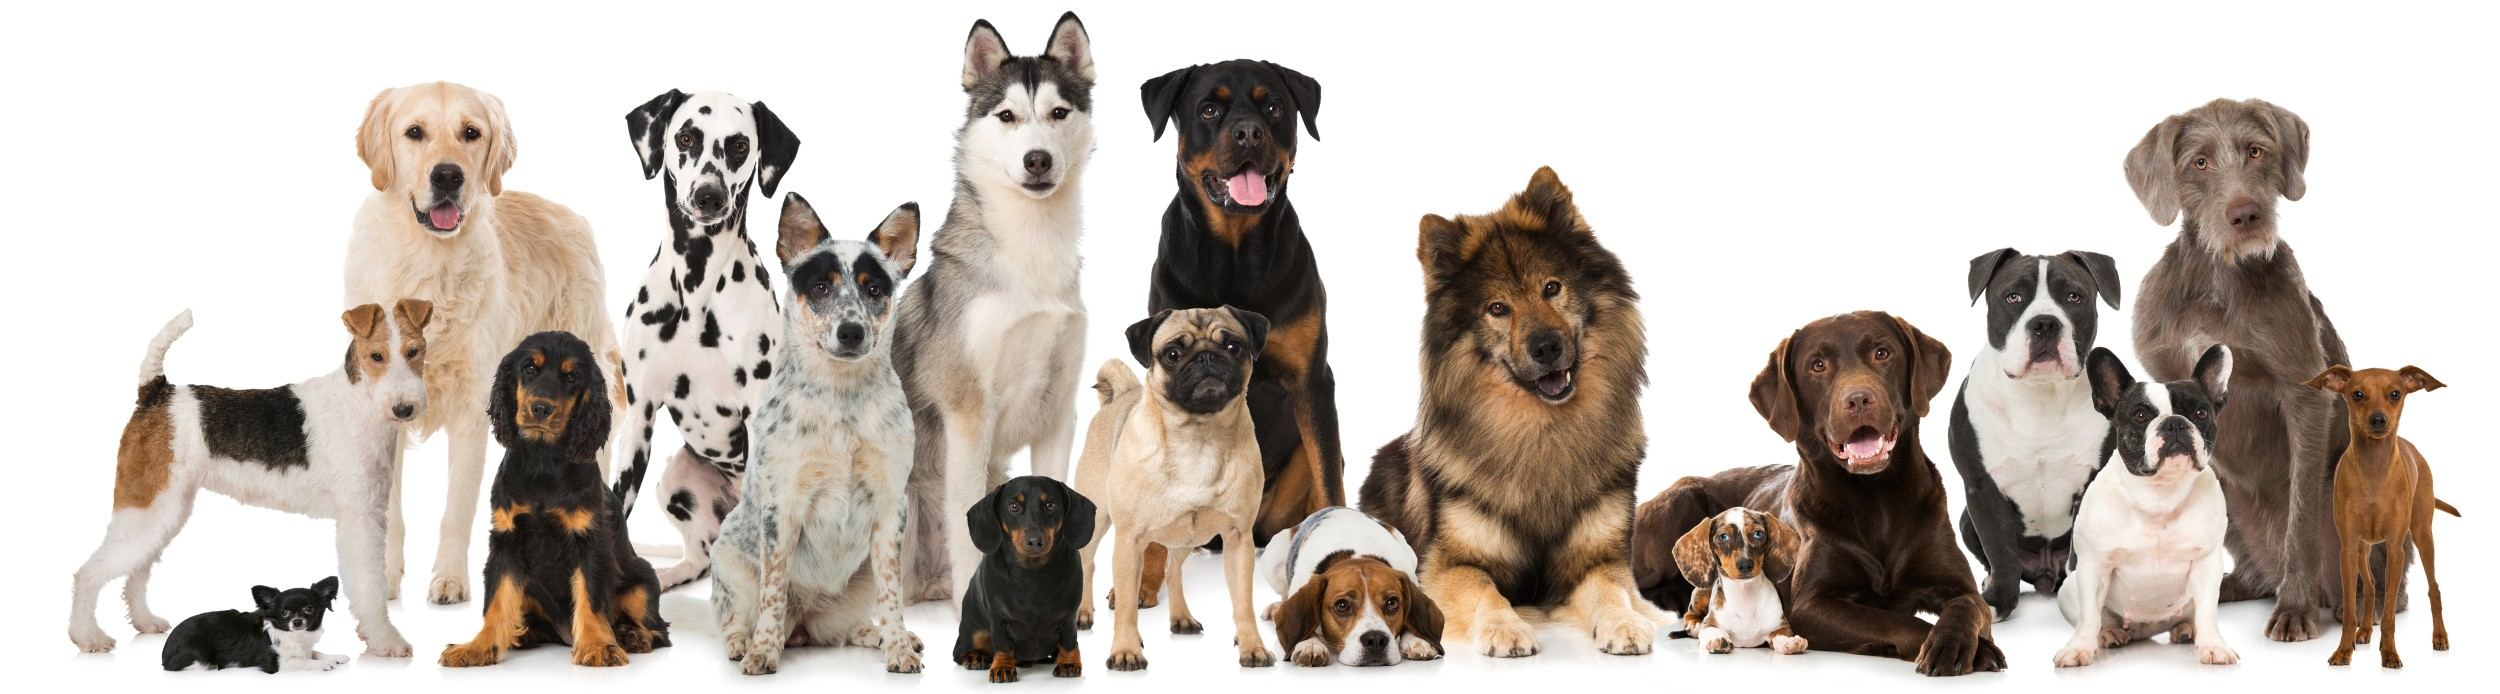
\includegraphics[width=8cm]{Figuras/caes}
            \caption[\small Algumas raças caninas com outro tamanho.]{\small Algumas raças caninas com outro tamanho\footnotemark.}
    	\label{fig_caes_com_foot}
    \end{figure}

    \begin{figure}[htp]
         \centering
         \begin{subfigure}[b]{0.3\textwidth}
             \centering
             
\includegraphics[width=\textwidth]{Figuras/buldog}
             \caption{}
             \label{fig:a}
         \end{subfigure}
         \hfill
         \begin{subfigure}[b]{0.3\textwidth}
             \centering
             
\includegraphics[width=\textwidth]{Figuras/shih_tzu}
             \caption{}
             \label{fig:b}
         \end{subfigure}
         \hfill
         \begin{subfigure}[b]{0.3\textwidth}
             \centering
             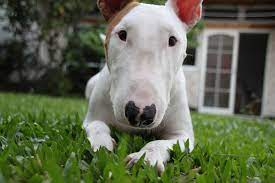
\includegraphics[width=\textwidth]{Figuras/bull_terrier}
             \caption{}
             \label{fig:c}
         \end{subfigure}
            \caption{\small Três raças de cães. (a) Bulldog; (b) Shih Tzu; (c) Bull Terrier.}
            \label{fig_c}
    \end{figure}
    
    Na Figura~\ref{fig_caes_sem_foot} são ilustradas algumas raças caninas. Na Figura~\ref{fig_caes_com_foot} é apresentada a figura anterior com a inclusão de uma nota de rodapé. As duas figuras apresentam duas formatações possíveis para o tamanho da figura. Na Figura~\ref{fig_caes_sem_foot}, o tamanho da imagem é definido relativamente à largura do texto (neste caso corresponde a 80\% da largura do texto). Já na Figura~\ref{fig_caes_com_foot}, a figura tem a largura absoluta de $8~cm$.   
    Um exemplo onde são colocadas três imagens lado a lado, indicando a referência de cada uma das imagens recorrendo a um só  \textit{label}, está apresentado na Figura~\ref{fig_c}. Na Figura~\ref{fig:b} pode visualizar-se um cão da raça Shih Tzu.
    
    \footnotetext{Fonte: \textit{https://images.app.goo.gl/HhdCXAy6DVtBYjsF9}}
    
    